\chapter{$\Na/\K$ pump (Na/K-ATPases)}
\label{chap:NaK_pump}

$\Na$,$\K$-ATPase is an important enzyme, responsible for maintaining $\Na$ and
$\K$ electrochemical potential gradients across the plasma membranes
(Sect.\ref{sec:NaK_pump}).
The enzyme's complete reaction cycle is widely based on Albers-Post formalism
(Sect.\ref{sec:nak-pump:-post}). 

Compare to ion channels, the individual pump produces a relatively slow ion flux
across the membrane. Thus, the measurement of ion pump kinetics, particular
partial reactions, have been limited to tissues with high level of expression of
these pumps, e.g. mammalian kidney \citep{jorgensen1974, jorgensen1974i},
with some in red blood cells and resealed red cell ghosts \citep{sachs1989}.

Recent studies showed that the kinetics of the enzyme (pump) in kidney is not
the same as that in cardiac cells. The related enzyme, e.g. SERCA, also differ
significantly between skeletal muscle and heart muscle \citep{cable1988}. 


The $\Na$ ions is believed to play important role in the initial phase
of AP. The Na/K exchanger pumps 3 Na out and 2 K in for each ATP
molecule that is hydrolized. So, The $I_\NaK$ is an outward current,
i.e. hyperpolarizing. Other names are {\bf electrogenic}
(electricity-generating) pump and less commonly, though arguably more
correctly, as a {\bf rheogenic} (current generating) pump.

After the rapid increase $[\Na]_i$ in the early phase of AP, we
observe a hyperpolarization - early after depolarization
(EAD). However, using Li instead of $\Na$, we don't see such
hyperpolarization. So, this can be explained as the increase activity
of $\NaK$ exchanger. Another test is to decrease extracellular
$[\Na]$, then inhibit the pump by using $\K$ free solution. Then, if
we restore extracellular $\K$, the pump start activating, and pump
$\Na$ out, causing a hyperpolarization.

The $I_\Na$ (inward) current occur at resting condition, so there must
be a exchanger flux to balance that. Under the experiment to inhibit
the exchanger, we observe a longer AP, i.e. more $\Na$ inside the
cell. 

The dependence of $\NaK$ exchanger on 
\begin{enumerate}
\item $[\Na]_i$ ? - NO, at a fixed $[\K]_o$, the rate constant for
  $\Na$ extrusion doesn't vary with intracellular $\Na$ activity
  ($a^i_\Na$). 


\item $[\K]_o$ ? - 
\end{enumerate}


% \section{Na/K pump}
% \label{sec:nak-pump}



\section{Chapman et al. (1979)}
\label{sec:nak-pump:-chapman}

\section{Difrancesco-Noble (1985)}

\citep{difrancesco1985mcea} use an electrogenic pump model, i.e. the pump
contribute to the formation of the potential gradient with Na:K stoichiometry of
3:2. 
\begin{equation}
I_p = i_p \frac{[\K]_o}{K_{m,\k}+[\K]_o} \frac{[\Na]_i}{K_{m,\na}+[\Na]_i}
\end{equation}
with the maximum current $i_p=125$nA and specified cell surafe area of
0.063cm$^2$, so the current per unit area is 0.02$\mum/$mm$^2$. 



\section{Lauger-Apel (1986)}
\label{sec:nak-pump:-lauger}


\section{Post-Albers (1989)}
\label{sec:nak-pump:-post}

Post-Albers is a consecutive ``ping-pong'' mechanism in which only one
(either $\Na$ or $\K$) can bind to the enzyme at a given
time~\citep{apell1989}. There can be other intermediate enzymes
complexes, with partial reaction steps. The basic mechanism of
Post-Albers is given in Fig.~\ref{fig:Post-Albers_NaK}. Here, E, P-E,
and ATP-E represent native, phosphorylated, and ATP-bound of the
enzyme. The subscript $i$ and $e$ denotes conformation in which the
cation binding sites is exposing to the cytosol, and extracellular
medium, respectively. 

\begin{figure}[hbt]
  \centerline{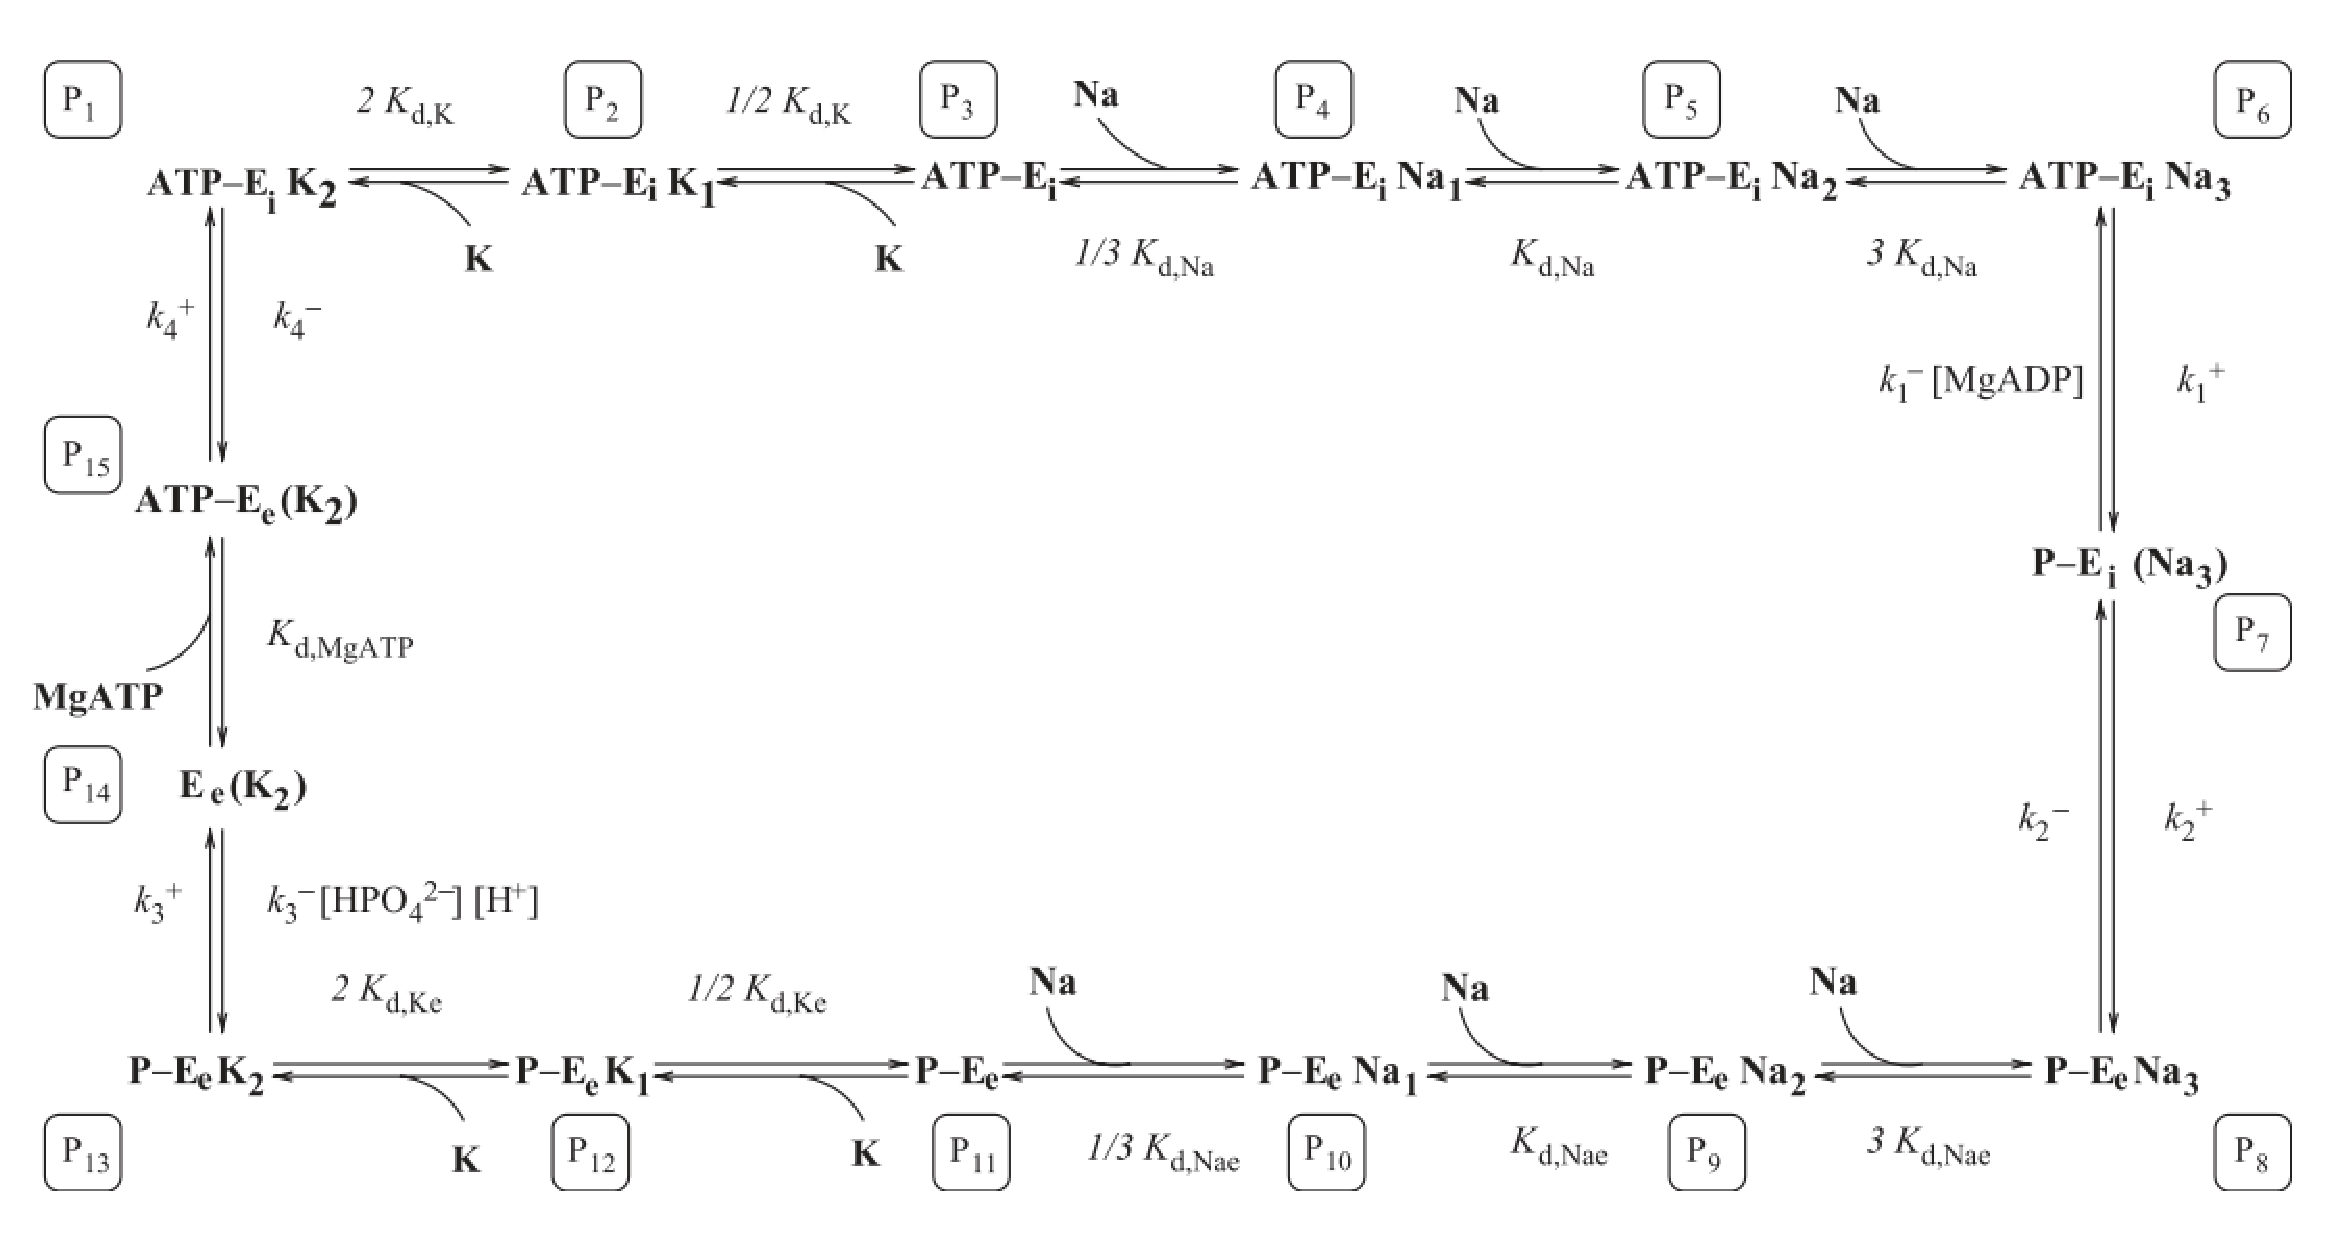
\includegraphics[height=6.6cm,
    angle=0]{./images/Post-Albers_NaK.eps}}
\caption{15-state Post-Albers reaction cycle for Na/K pump}
\label{fig:Post-Albers_NaK}
\end{figure}

If the dissociation for the binding of a cation is $K_d$, and the
binding is consecutive; then the $m$-th ion binding to one of the $n$
identical binding sites has the dissociation constant
$\frac{mK_d}{n-m+1}$. In Fig.~\ref{fig:Post-Albers_NaK}, 
\begin{itemize}
\item ion binding/unbinding and binding of MgATP, those without the
  forward/reverse rate constants $k^+, k^-$, are assumed to be rapid
  reactions, with dissociation constant $K_d$.

\item conformation changes ($E_i$ to $E_e$ and vice versa), reactions
  with metabolites are not considered rapid. 
\end{itemize}

Another simplification is that the three $\Na$ binding sites, as well
as the two $\K$ binding sites, are identical and independent.

\begin{equation}
  \label{eq:1177}
  \ce{MgATP + H2O <=>[K_{MgATP}] MgADP + Pi + H+}
\end{equation}

The free energy released by the hydrolysis of ATP, $\Delta G_{MgATP}$
which is determined as
\begin{equation}
  \label{eq:1178}
  \Delta G_{MgATP} = \Delta G^\circ_{MgATP} + RT\ln\frac{[\MgADP][\Pi][\H]}{[\MgATP]}
\end{equation}
with $\Delta G^\circ_\MgATP$ is the free energy under standard
condition. 
\begin{equation}
  \label{eq:1179}
  \Delta G^\circ_\MgATP = -RT \ln K_\MgATP
\end{equation}
NOTE: Under normal condition, $\Delta G^\circ \sim -58$kJ.mol$^{-1} < 0$,
meaning ATP hydrolysis is exergonic (i.e. energy release)~\citep{ingwall2002}. 

Suppose the energy required to translocate a $\K$ ion from
extracellular medium to inside is $\Delta G_K$ (against the
electrochemical gradient)
\begin{equation}
  \label{eq:1180}
  \Delta G_K = RT \ln \frac{[\K_i]}{[\K_e]} + FV_m
\end{equation}
The first term accounts for the movement against the concentration
gradient, and the second term accounts for the movement of the charge
through the membrane potential $V_m$

The energy required to translocate a $\Na$ ion from intracellular to
outside is $\Delta G_\na$
\begin{equation}
  \label{eq:1181}
  \Delta G_\na = RT \ln \frac{[\Na_e]}{[\Na_i]} - FV_m
\end{equation}
with $V_m \sim -85$mV. 

So, the energy required per pump cycle, $\Delta G_\text{pump}$ is
\begin{equation}
  \label{eq:1182}
  \Delta G_\text{pump} = 2\Delta G_\K + 3\Delta G_\na
\end{equation}
\begin{framed}
  The pump current direction can be determined using purely
  thermodynamics (second law). If $-\Delta G_\MgATP > \Delta
  G_\text{pump}$ the pump works in forward direction. If $\Delta
  G_\MgATP + \Delta G_\text{pump} = 0$, the pump is in equilibrium,
  and the net transport is zero. If $\Delta G_\MgATP + \Delta
  G_\text{pump} < 0$, the pump operates in reverse mode.

  Reverse mode have been reported in erythrocyte (red blood
  cells)~\citep{lew1970}. 
\end{framed}

Using~\citep{hill1989} approach, the 15-step cycle, at equilibrium,
has
\begin{equation}
  \label{eq:1186}
  \frac{k^+_1k^+_2k^+_3k^+_4K^2_{d,K_i}K^3_{d,\na_e}}{k^-_1k^-_2k^-_3k^-_4K_{d,\MgATP}K^2_{d,\k_e}K^2_{d,\na_i}}
  = \frac{[\MgADP][\Pi][\H][\k_i]^2[\na_e]^3}{[\MgATP][\k_e]^2[\na_i]^3}
\end{equation}
Also, at equilibrium, we have $\Delta G_\MgATP + \Delta G_\text{pump}
= 0$, so
\begin{equation}
  \label{eq:1187}
  -\ln K_\MgATP + \ln \frac{[\MgADP][\Pi][\H]}{[\MgATP]} + 3\ln
  \frac{[\na_e]}{[\na_i]} + 2 \ln
  \frac{[\k_i]}{[\k_e]}-\frac{FV_m}{RT}  = 0
\end{equation}
taking the exponential, then 
\begin{equation}
  \label{eq:1188}
  \frac{[\MgADP][\Pi][\H][\na_e]^3[\k_i]^2}{[\MgATP][\na_i]^3[\k_e]^2}   =  K_\MgATP\exp\{FV_m/(RT)\}
\end{equation}

Finally, combine eq.~\eqref{eq:1186} and eq.~\eqref{eq:1188}, the
transition rates must satisfy a voltage-dependent
\begin{equation}
  \label{eq:1189}
  \frac{k^+_1k^+_2k^+_3k^+_4K^2_{d,K_i}K^3_{d,\na_e}}{k^-_1k^-_2k^-_3k^-_4K_{d,\MgATP}K^2_{d,\k_e}K^2_{d,\na_i}}
  =  K_\MgATP\exp\{FV_m/(RT)\}
\end{equation}


\begin{framed}
  Based on ~\citep{hill1989}, an examination at thermodynamics
  equilibrium reveals a thermodynamics constraint on the kinetic
  parameters for the scheme. 
  \begin{equation}
    \label{eq:1183}
    k^+_i P_i = k^-_i P_{i+1}
  \end{equation}
  with $P_i, P_{i+1}$ are fractional occupancies of adjacent states,
  $k^+, k^-$ are first-order rate constants. For a $n$-step cycle, the
  product on one direction should be equal to the product on the
  reverse one.
  \begin{equation}
    \label{eq:1184}
    \prod_{i=1}^n k^+_i P_i = \prod_{i=1}^n k^-_i P_{i+1}
  \end{equation}
  where $P_{n+1} = P_1$. or simply $ \prod_{i=1}^n k^+_i = \prod_{i=1}^n
  k^-_i $. As the state occupancies are canceled out, this constraints
  for the kinetic parameters must hold whether or not the system is at
  equilibrium. 

  For a transition that involves ion bind or unbind from the enzyme,
  eq.~\eqref{eq:1183} can be written as
  \begin{equation}
    \label{eq:1185}
    k^+_i [Y]P_i = k^-_i P_{i+1}
  \end{equation}
  with $k^+_i$ now is a second-order rate constants. 
\end{framed}

For the above examination to be valid, the pump cycle must be
unbranched kinetic cycle, i.e. there is no transition between states
not linked in Fig.~\ref{fig:Post-Albers_NaK}. To further justify the
affect of $V_m$ on sodium transport, we have
\begin{equation}
  \label{eq:1190}
  \frac{k^+_1k^+_2k^+_3k^+_4K^2_{d,K_i}(K^O_{d,\na_e})^3}{k^-_1k^-_2k^-_3k^-_4K_{d,\MgATP}K^2_{d,\k_e}(K^O_{d,\na_i})^2}
  =  K_\MgATP
\end{equation}
with
\begin{equation}
  \label{eq:1191}
  \begin{split}
    K_{d,\na_e}= K^O_{d,\na_e}\exp\{(\Delta-1)FV_m/(3RT)\} \\
    K_{d,\na_i}= K^O_{d,\na_e}\exp\{(\Delta)FV_m/(3RT)\} \\
  \end{split}
\end{equation}
where $K^O_{d,\na_e},K^O_{d,\na_i}$ are $\Na$ dissociation constants
at $V_m=0$ and the factor $\Delta$ determines how the voltage
dependence is partitioned between the intra- and extra-cellular $\Na$
dissociation reactions. Typically, we can choose $\Delta =1/2$. 

\section{Smith-Crampin (2004)}
\label{sec:nak:-smith-crampin}

Even though Na/K pumps model are electrogenic and is dependent on free
energy of ATP hydrolysis, so far, models has not incorporated
metabolite dependence into their parameters, i.e. metabolite
concentration need to be a variable in the model.

Under physiological conditions, ATP concentration, and free energy
associated with ATP hydrolysis, remain approximately
constant. However, under pathological condition, e.g. ischaemia when
the drop in free energy may cause the pump to stop or function in
reverse mode.

The energy required is typically 17\% of ATP
turnover~\citep{schram1994}. The coupling ratio is 3$\Na$ out + 2 $\K$
in, for each ATP hydrolyzed~\citep{glitsch2001}. So, the net transport
is one charge out of the cell for each ATP consumption.
\begin{equation}
  \label{eq:1176}
  \ce{ATP + 3Na+_i + 2K+_e <=> ADP + Pi + 3Na+_e + 2K+_i}
\end{equation}

\begin{framed}
  The reduction of energy may cause an increase of $[\Na]_i$, which
  directly reduce Na/Ca exchanger activity. Finally, it increase
  $[\Ca]_i$, and drop in pH (via reduce Na/H
  exchange)~\citep{ingwall2002}. This increase the contraction of the
  cell may lead to disruption regulation of cell volume and
  intracellular calcium handling.
\end{framed}


Based on the model described in
Sect.~\ref{sec:nak-pump:-post} and apply the reduction technique for
equilibrium reactions in
Sect.~\ref{sec:equil-appr},~\citep{smith2004} induced a new
kinetics scheme in Fig.~\ref{fig:SmithCrampin_NaK}. 

\begin{figure}[hbt]
  \centerline{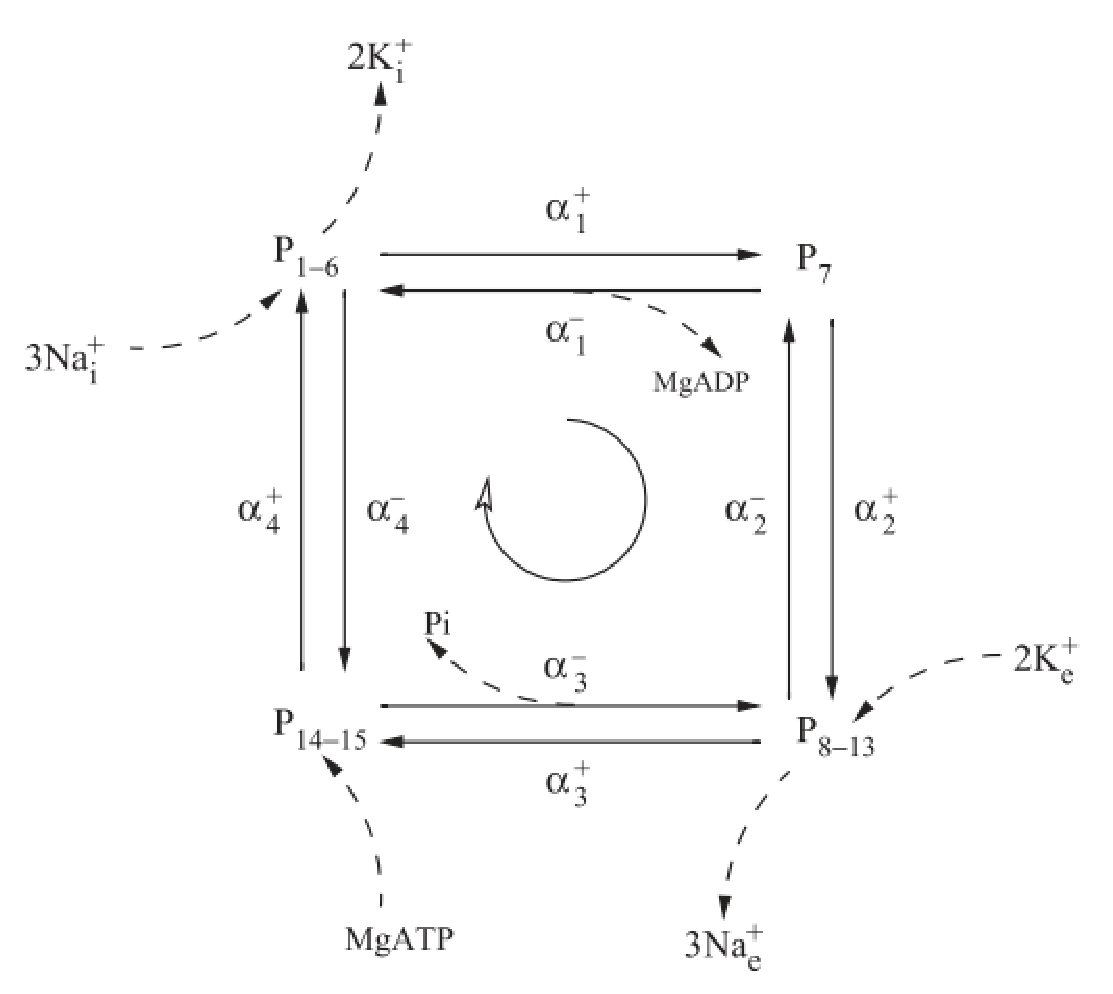
\includegraphics[height=5cm,
    angle=0]{./images/SmithCrampin_NaK.eps}}
 \caption{A reduced scheme for Na/K-ATPase. The ion, metabolite
   binding/unbinding are groupped into the pseudo first-order reaction
 constant $\alpha^\pm_j$}
\label{fig:SmithCrampin_NaK}
\end{figure}
The forward reaction constants (in clockwise) are
\begin{equation}
  \label{eq:1201}
  \begin{array}{ll}
    \alpha^+_1 = \frac{}{} & \alpha^+_2 = k^+_2 \\
    \alpha^+_3 = \frac{}{} & \alpha^+_4 = \frac{}{}
  \end{array}
\end{equation}
The reverse reaction constants (in counter-clockwise) are
\begin{equation}
  \label{eq:1202}
  \begin{array}{ll}
    \alpha^-_1 = \frac{}{} & \alpha^-_2 = \frac{}{} \\
    \alpha^-_3 = \frac{}{} & \alpha^-_4 = \frac{}{}    
  \end{array}
\end{equation}

For a simple cycle with no branching, the steady-state flux ...


The steady-state cycle rate can be solved
\begin{equation}
  \label{eq:1203}
  v_{\text{cyc},\NaK} = \frac{}{\sum}
\end{equation}
with $\sum$ is the sum of 16 product terms.
Thus, the whole-cell pump current density $i_\NaK$ is
\begin{equation}
  \label{eq:1204}
  i_\NaK = v_{\text{cyc},\NaK} .F. \rho_\NaK
\end{equation}
with $\rho_\NaK$ is the density of the Na/K-ATPase proteins in the
sarcolemma. 


\section{Garcia-\ldots-Clarke (2012)}

\citep{garcia2012}


